% w nawiasie kwadratowym wpisujemy rodzaj pracy: 
% magisterska, licencjacka, inzynierska
\documentclass[magisterska]{pracadypl}

%% ważne definicje %%
\usepackage{tgtermes}
\usepackage[T1]{fontenc}
\usepackage{polski}
\usepackage[utf8]{inputenc}
\input glyphtounicode
\pdfgentounicode=1
\usepackage{amssymb}
\usepackage{amsmath}
\usepackage{caption}
\usepackage{graphicx}
\setcounter{secnumdepth}{4}  % Ensure subsubsection is numbered
\setcounter{tocdepth}{4}     % Ensure subsubsection appears in TOC
\usepackage{titlesec}
\usepackage{color}
\usepackage{xcolor}
\usepackage{float}
\usepackage{listings}
\usepackage{parskip}
\usepackage{xcolor} % optional, for color
\usepackage{chngcntr}
\counterwithout{figure}{chapter}
\bibliographystyle{plain}

\def\mgr{magisterska}
\def\lic{licencjacka}
\def\inz{inżynierska}

\def\sk{Słowa kluczowe}
\def\kw{Keywords}
\def\et{Title in English}
%% koniec ważnych definicji %%

%% wypełnia Autor pracy %%

%autor pracy
\author{Gabriel Ozeg}
%numer albumu
\nralbumu{395263}
%tytuł pracy
\title{System antykolizyjny na mikroprocesorze Raspberry Pi}
%kierunek studiów
\kierunek{Informatyka}
%promotor w dopełniaczu
\opiekun{dr Paweł Zajączkowski}
\katedra{Katedra Informatyki Stosowanej}
%rok
\date{2025}
%Słowa kluczowe:
\slkluczowe{Przetwarzanie obrazu, Głębia obrazu, Metody pomiaru odległości w czasie rzeczywistym, Zastosowania w robotyce}
%tytuł po angielsku
\tytulang{Collision avoidance system on Raspberry Pi microprocessor}
%słowa kluczowe po angielsku
\keywords{Image Processing, Image Depth, Real-Time Distance Measurement Methods, Applications in Robotics}
%% koniec ważnych definicji %%

%% APD %%
%% w systemie APD należy jeszcze wpisać, poza powyższymi informacjami, streszczenie oraz streszczenie w języku angielskim  %%


%%% definicje %%%
\def\pd{\noindent \textbf{Dowód.~}} %%początek dowodu
\def\kd{\hfill\mbox{$\rule{2mm}{2mm}$}} %%koniec dowodu
\newtheorem{defi}{Definicja}[section]
\newtheorem{uwaga}{Uwaga}[section]
\newtheorem{tw}{Twierdzenie}[section]
\newtheorem{lem}{Lemat}[section]
\newtheorem{wn}{Wniosek}[section]
\renewcommand\thetw{\thesection.\arabic{tw}.}
\renewcommand\thedefi{\thesection.\arabic{defi}.}
\renewcommand\theuwaga{\thesection.\arabic{uwaga}.}
\renewcommand\thetw{\thesection.\arabic{tw}.}
\renewcommand\thelem{\thesection.\arabic{lem}.}
\renewcommand\thewn{\thesection.\arabic{wn}.}
%
\definecolor{wmiigreen}{rgb}{0.0, 0.5, 0.0}
\titleformat{\chapter}[display]
  {\normalfont\huge\bfseries\color{wmiigreen}}{\chaptertitlename\ \thechapter}{10pt}{\Huge}
 %
\linespread{1.3}
%%% koniec definicji %%%

\begin{document}

\lstdefinestyle{mypython}{
    language=Python,
    basicstyle=\ttfamily\scriptsize,
    keywordstyle=\color{red}\bfseries,
    stringstyle=\color{green},
    commentstyle=\color{blue},
    inputencoding=utf8,
    literate=
      {ą}{{\k{a}}}1 {Ą}{{\k{A}}}1
      {ć}{{\'c}}1 {Ć}{{\'C}}1
      {ę}{{\k{e}}}1 {Ę}{{\k{E}}}1
      {ł}{{\l{}}}1 {Ł}{{\L{}}}1
      {ń}{{\'n}}1 {Ń}{{\'N}}1
      {ó}{{\'o}}1 {Ó}{{\'O}}1
      {ś}{{\'s}}1 {Ś}{{\'S}}1
      {ź}{{\'z}}1 {Ź}{{\'Z}}1
      {ż}{{\.z}}1 {Ż}{{\.Z}}1
}

\maketitle
\tableofcontents
\newpage

\chapter{Wstęp}

Przetwarzanie obrazu cyfrowego stanowi jedną z kluczowych dziedzin współczesnej informatyki oraz inżynierii komputerowej, znajdującą zastosowanie w wielu obszarach życia codziennego, przemysłu i nauki. Głównym celem tej dziedziny jest analiza, przekształcanie oraz interpretacja danych wizualnych przy użyciu metod matematycznych, algorytmów komputerowych oraz technik sztucznej inteligencji. Przetwarzanie obrazu umożliwia nie tylko poprawę jakości obrazów, ale także automatyczną ekstrakcję informacji, segmentację obiektów, rozpoznawanie kształtów czy estymację głębi sceny.

Systemy wizyjne znajdują zastosowanie m.in. w diagnostyce medycznej (np. analiza obrazów RTG i MRI), przemyśle (automatyczna kontrola jakości), systemach bezpieczeństwa (rozpoznawanie twarzy i analiza zachowań) oraz w autonomicznych pojazdach i robotyce, gdzie odpowiadają za detekcję przeszkód i wspomaganie decyzji nawigacyjnych w czasie rzeczywistym. Szczególne znaczenie zyskują implementacje systemów wizyjnych na platformach o ograniczonych zasobach sprzętowych, takich jak mikrokontrolery czy komputery jednopłytkowe.

Celem niniejszego projektu jest implementacja oraz ocena działania \textbf{systemu antykolizyjnego} opartego na przetwarzaniu obrazu stereoskopowego w czasie rzeczywistym. Główną platformą obliczeniową jest \textbf{Raspberry Pi 5} – komputer jednopłytkowy nowej generacji, oferujący około 50\% wyższą wydajność w porównaniu do swojego poprzednika, co czyni go obiecującą jednostką dla zastosowań typu \textit{edge computing}.

System bazuje na wykorzystaniu \textbf{stereowizji}, czyli przetwarzania obrazu z dwóch zsynchronizowanych kamer w celu uzyskania mapy dysparycji i wyznaczenia odległości do obiektów w scenie. W przypadku wykrycia przeszkody znajdującej się zbyt blisko, system podejmuje decyzję o zatrzymaniu pojazdu poprzez fizyczne odłączenie zasilania jego silnika napędowego, co ma na celu uniknięcie kolizji.

Projekt został zrealizowany przy użyciu następujących komponentów sprzętowych:

\begin{itemize}
  \item \textbf{Raspberry Pi 5} – odpowiada za przetwarzanie obrazu stereoskopowego, analizę głębi oraz sterowanie logiką decyzyjną systemu.
    \begin{figure}[H]  % 'h' means "here", it places the figure at the current location in the document
      \centering  % Centers the image
      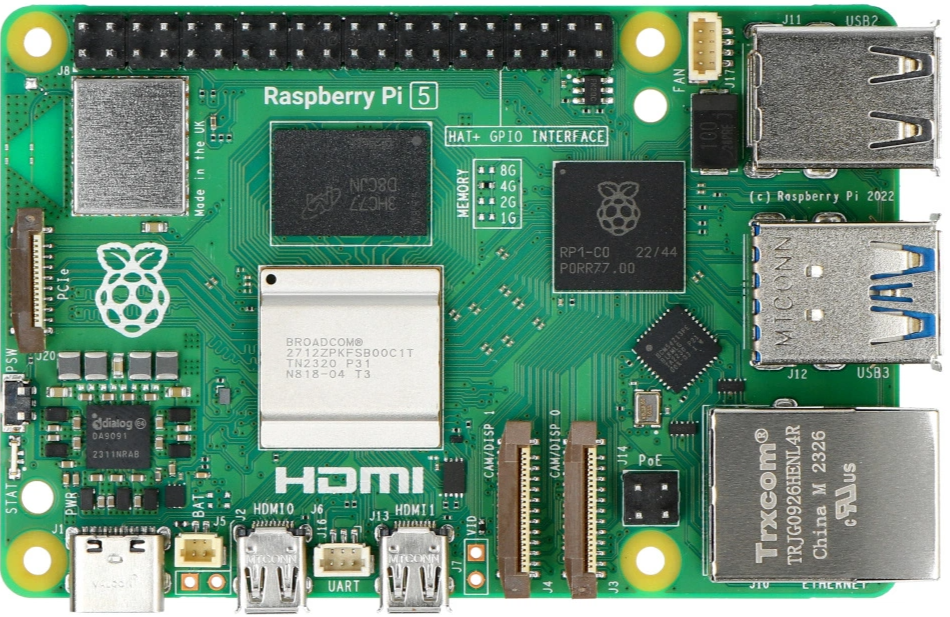
\includegraphics[width=0.5\textwidth]{images/rpi5.png}  % Adjust the path and width as necessary
      \captionsetup{font=footnotesize}
      \caption[Płytka Raspberry Pi 5. https://www.hackatronic.com/wp-content/uploads/2024/03/Raspberry-Pi-5-Pinout--1210x642.jpg]{Płytka Raspberry Pi 5.}
    \end{figure}

  \item \textbf{Kamera stereo} – dostarcza zsynchronizowane obrazy z dwóch perspektyw, umożliwiające wyznaczenie mapy głębi.
    \begin{figure}[H]  % 'h' means "here", it places the figure at the current location in the document
      \centering  % Centers the image
      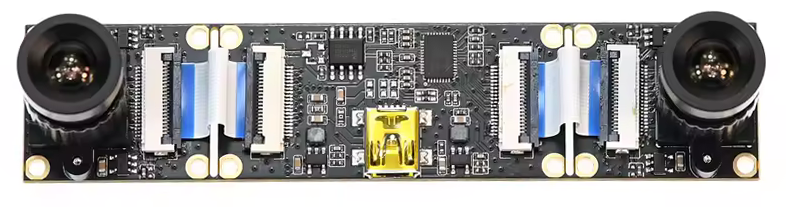
\includegraphics[width=0.5\textwidth]{images/MAINSTEREO.png}  % Adjust the path and width as necessary
      \captionsetup{font=footnotesize}
      \caption[Kamera stereowizyjna. https://cell-kom.com/inne/21454-kamera-internetowa-full-hd-b16-1080p-5900217390350.html]{Kamera stereowizyjna}
      \label{fig:mono}  % Optional: use to refer to this image later in the text
    \end{figure}

  \item \textbf{Moduł UPS HAT (B) firmy Waveshare} – zapewnia nieprzerwane zasilanie, umożliwiając pracę systemu w warunkach mobilnych oraz zwiększając jego niezawodność.
    \begin{figure}[H]  % 'h' means "here", it places the figure at the current location in the document
      \centering  % Centers the image
      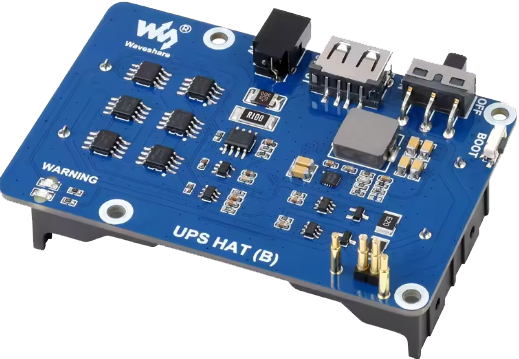
\includegraphics[width=0.5\textwidth]{images/upsfront.png}  % Adjust the path and width as necessary
      \captionsetup{font=footnotesize}
      \caption[Moduł zasilający. https://www.waveshare.com/wiki/UPS-HAT-(B)]{Moduł zasilający.}
    \end{figure}

  \item \textbf{Moduł przekaźnikowy} – odpowiada za fizyczne odłączenie zasilania jednostki napędowej w przypadku wykrycia zagrożenia kolizją.

    \begin{figure}[H]  % 'h' means "here", it places the figure at the current location in the document
      \centering  % Centers the image
      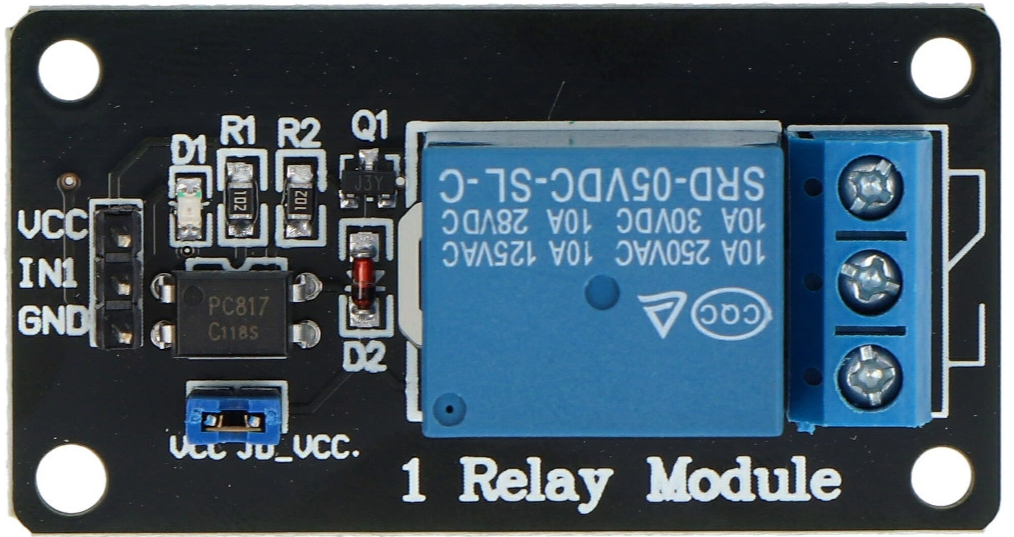
\includegraphics[width=0.4\textwidth]{images/relay.png}  % Adjust the path and width as necessary
      \captionsetup{font=footnotesize}
      \caption[Moduł przekaźnika. https://l1nq.com/hQOm9]{Moduł przekaźnika.}
    \end{figure}

  \item \textbf{Zabawkowy samochód elektryczny} – służy jako platforma testowa dla systemu, umożliwiając przeprowadzanie eksperymentów w warunkach laboratoryjnych oraz polowych.
    \begin{figure}[H]  % 'h' means "here", it places the figure at the current location in the document
      \centering  % Centers the image
      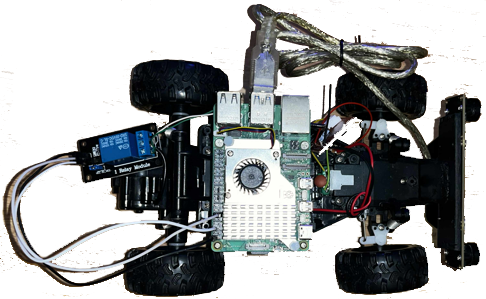
\includegraphics[width=0.4\textwidth]{images/auto.png}  % Adjust the path and width as necessary
      \captionsetup{font=footnotesize}
      \caption[Pojazd projektu. Opracowanie własne]{Pojazd projektu.}
    \end{figure}

\end{itemize}

W ramach realizacji projektu przeprowadzona została analiza skuteczności oraz wydajności systemu w warunkach rzeczywistych. Zakres badań obejmował:

\begin{itemize}
  \item ocenę dokładności estymacji głębi oraz detekcji przeszkód,
  \item pomiar obciążenia obliczeniowego Raspberry Pi 5 i ocena jego zdolności do pracy w czasie rzeczywistym,
  \item analizę responsywności systemu w kontekście szybkości reakcji na przeszkody,
  \item testy stabilności zasilania przy wykorzystaniu UPS HAT w środowisku mobilnym,
  \item ocenę możliwości zastosowania projektu w celach komercyjnych, m.in. w robotyce mobilnej, pojazdach magazynowych czy inteligentnych systemach bezpieczeństwa.
\end{itemize}

Implementacja systemu antykolizyjnego na bazie Raspberry Pi 5 oraz kamery stereoskopowej wykazała, że nawet przy ograniczonych zasobach sprzętowych możliwe jest skuteczne przeprowadzanie przetwarzania obrazu w czasie rzeczywistym. Pomimo istotnego obciążenia obliczeniowego, stereowizja dostarcza bogatych informacji o głębi sceny, co zwiększa niezawodność systemów unikania przeszkód.

Dzięki kompaktowym rozmiarom, niskiej cenie oraz energooszczędności, Raspberry Pi 5 okazuje się atrakcyjną platformą dla zastosowań edukacyjnych, prototypowych oraz potencjalnie komercyjnych.

\chapter{Natura kamery}

Kamery rejestrują promienie świetlne z otoczenia. Zasadniczo kamera działa podobnie jak ludzkie oko — odbite promienie światła trafiają do oka i są skupiane na siatkówce.

Najprostszym modelem kamery jest tzw. „kamera otworkowa” \cite{otworkowa}. To dobre uproszczenie pozwalające zrozumieć podstawy działania kamery. W tym modelu wszystkie promienie świetlne są blokowane przez ścianki, a tylko te przechodzące przez mały otwór trafiają na powierzchnię światłoczułą wewnątrz kamery, tworząc odwrócony obraz. Poniższa ilustracja przedstawia tę zasadę.

\begin{figure}[H]
    \centering
    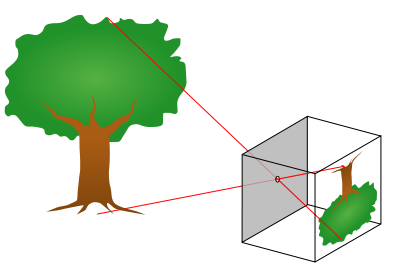
\includegraphics[width=0.5\textwidth]{images/light.png}
    \captionsetup{font=footnotesize}
    \caption[Odwrócenie obrazu przez soczewkę. https://funsizephysics.com/use-light-turn-world-upside/]{Odwrócenie obrazu przez soczewkę}
    \label{fig:rpi}
\end{figure}

Choć ten model jest prosty, nie nadaje się dobrze do rejestrowania wystarczającej ilości światła przy krótkim czasie naświetlania. Dlatego w kamerach stosuje się soczewki, które skupiają promienie świetlne w jednym punkcie. Niestety, powoduje to powstawanie zniekształceń.

Istnieją dwa główne rodzaje zniekształceń:

\begin{itemize}
  \item Zniekształcenie promieniowe(radialne) — spowodowane kształtem soczewki,występujące symetrycznie względem środka obrazu.

  \item Zniekształcenie styczne(tangencjalne) — wynikające z niedoskonałości montażu lub geometrii kamery.
\end{itemize}

Obrazy zniekształcone w ten sposób można skorygować za pomocą metod matematycznych. Proces kalibracji pozwala stworzyć model geometrii kamery oraz model zniekształceń obiektywu. Te modele określają tzw. parametry wewnętrzne kamery.

\section{Ogniskowa obiektywu}

Względny rozmiar obrazu rzutowanego na powierzchnię w kamerze zależy od ogniskowej \cite{ogniskowa}.

W modelu otworkowym ogniskowa to odległość między otworem, przez który przechodzi światło, a obszarem, na który rzutowany jest obraz.

Aby wyznaczyć, jak duży będzie obraz obiektu na płaszczyźnie projekcji, korzystamy z \textbf{twierdzenia Talesa}.  
Dlaczego?

Obiekt znajdujący się w przestrzeni oraz jego rzut w kamerze tworzą dwa \textbf{podobne trójkąty}:
\begin{itemize}
    \item Jeden utworzony przez obiekt o wysokości \( X \), znajdujący się w odległości \( Z \) od kamery.
    \item Drugi utworzony przez obraz tego obiektu na płaszczyźnie znajdującej się w odległości \( f \) od otworu kamery, którego wysokość to \( x \).
\end{itemize}

Ponieważ kąty tych trójkątów są identyczne (wierzchołek kąta w otworze kamery) i odpowiadające sobie boki są proporcjonalne, możemy zastosować twierdzenie Talesa:

\[
\frac{x}{f} = \frac{X}{Z} \Rightarrow x = f \cdot \frac{X}{Z}
\]

Obraz na matrycy jest odwrócony, dlatego często w literaturze pojawia się wersja ze znakiem minus:

\[
-x = f \cdot \frac{X}{Z}
\]

\begin{itemize}
  \item \textbf{$x$}: obraz obiektu (znak minus wynika z tego, że obraz jest odwrócony)
  \item \textbf{$X$}: rozmiar obiektu
  \item \textbf{$Z$}: odległość od otworu do obiektu
  \item \textbf{$f$}: ogniskowa, odległość od otworu do obrazu
\end{itemize}

\begin{figure}[H]  % 'h' means "here", it places the figure at the current location in the document
    \centering  % Centers the image
    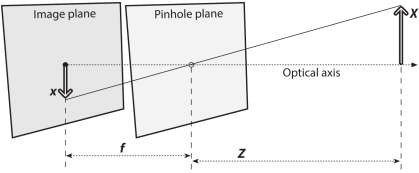
\includegraphics[width=0.5\textwidth]{images/pinhole.png}  % Adjust the path and width as necessary
    \captionsetup{font=footnotesize}
    \caption[Model kamery otworkowej. Learning OpenCV 3, O'Reilly, Str. 639]{Model kamery otworkowej}
    \label{fig:rpi}  % Optional: use to refer to this image later in the text
\end{figure}

Ponieważ soczewka nie jest idealnie wyśrodkowana, wprowadzono dwa parametry, $C_x$ i $C_y$, oznaczające odpowiednio poziome i pionowe przemieszczenie soczewki.
Ogniskowa na osiach $X$ i $Y$ są również różna, ponieważ obszar obrazu jest prostokątny. Daje to następujący wzór na położenie obiektu na powierzchni.

\[
x_{\text{screen}} = f_x \left( \frac{X}{Z} \right) + c_x, \quad
y_{\text{screen}} = f_y \left( \frac{Y}{Z} \right) + c_y
\]

Rzutowane punkty świata rzeczywistego na powierzchnię obrazu można zatem modelować w następujący sposób. $M$ jest tutaj macierzą wewnętrzną.

\bigskip

Punkt w przestrzeni 3D:
\[
Q = \begin{bmatrix} X \\ Y \\ Z \end{bmatrix}
\]

Po rzutowaniu za pomocą macierzy kamery $M$:
\[
M = \begin{bmatrix}
f_x & 0 & c_x \\
0 & f_y & c_y \\
0 & 0 & 1
\end{bmatrix}
\]

otrzymujemy punkt obrazu w jednorodnych współrzędnych:
\[
q = M \cdot \begin{bmatrix}
\frac{X}{Z} \\
\frac{Y}{Z} \\
1
\end{bmatrix}
=
\begin{bmatrix}
f_x \cdot \frac{X}{Z} + c_x \\
f_y \cdot \frac{Y}{Z} + c_y \\
1
\end{bmatrix}
\]

Po normalizacji współrzędnych jednorodnych:
\[
x = \frac{q_x}{q_w} = f_x \cdot \frac{X}{Z} + c_x
\quad , \quad
y = \frac{q_y}{q_w} = f_y \cdot \frac{Y}{Z} + c_y
\]

Dla ogólnej macierzy projekcji:
\[
P = M \cdot [R \;|\; t]
\]

Macierz \( P = M[R | t] \) nazywana jest macierzą projekcji kamery i zawiera zarówno informacje o parametrach wewnętrznych kamery (macierz \( M \)), jak i jej położeniu i orientacji w przestrzeni (macierze \( R \) i \( t \)).

Rzut punktu \( Q_h = \begin{bmatrix} X \\ Y \\ Z \\ 1 \end{bmatrix} \) przy pomocy tej macierzy daje nam współrzędne punktu\\ \( q = \begin{bmatrix} x' \\ y' \\ w \end{bmatrix} \) w jednorodnych współrzędnych, które po znormalizowaniu (\( x = \frac{x'}{w} \)) dają końcowe położenie punktu na obrazie.

\[
x = \frac{x'}{w}, \quad y = \frac{y'}{w}
\]

Współrzędne \( x, y \) po normalizacji są współrzędnymi piksela na płaszczyźnie obrazu, czyli miejscem, gdzie dany punkt 3D zostanie odwzorowany na zdjęciu lub klatce z kamery. Uwzględniają one zarówno parametry geometryczne obiektywu (ogniskowe \( f_x, f_y \)) jak i przesunięcia optycznego środka obrazu (\( c_x, c_y \)).

\section{Dystorsja obrazu}

\begin{figure}[H]  % 'h' means "here", it places the figure at the current location in the document
    \centering  % Centers the image
    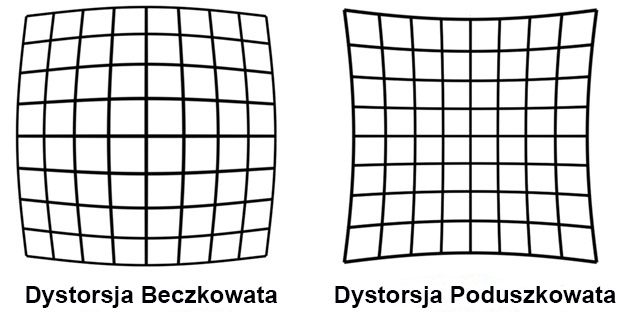
\includegraphics[width=0.5\textwidth]{images/dystorsje.png}  % Adjust the path and width as necessary
    \captionsetup{font=footnotesize}
    \caption[Rodzaje dystorsji. https://beafoto.pl/dystorsja]{Rodzaje dystorsji}
    \label{fig:rpi}  % Optional: use to refer to this image later in the text
\end{figure}

Teoretycznie możliwe jest zbudowanie obiektywu, który nie powoduje zniekształceń, np. przy użyciu soczewki parabolicznej. W praktyce jednak znacznie łatwiej i taniej jest wytwarzać soczewki sferyczne, które niestety powodują różne typy zniekształceń geometrycznych obrazu \cite{dystorsja}.

Aby móc opisać i skorygować te zniekształcenia, punkt obrazu wyrażony w pikselach \( (u, v) \) przekształca się najpierw do znormalizowanego układu współrzędnych kamery:

\[
x = \frac{u - c_x}{f_x}, \quad y = \frac{v - c_y}{f_y}
\]

Gdzie:
\begin{itemize}
    \item \( (c_x, c_y) \) — współrzędne głównego punktu optycznego (środka obrazu),
    \item \( (f_x, f_y) \) — ogniskowe w poziomie i pionie wyrażone w pikselach,
    \item \( (x, y) \) — znormalizowane współrzędne względem osi optycznej kamery.
\end{itemize}

\subsection*{Zniekształcenia promieniowe}

Zniekształcenia promieniowe (ang. \textit{radial distortion}) \cite{promieniowe} są symetryczne względem środka obrazu i ich wpływ rośnie wraz z odległością od środka. Dla punktów znormalizowanych odległość ta dana jest przez:

\[
r^2 = x^2 + y^2
\]

Efekt zniekształcenia można modelować jako nieliniową funkcję \( D(r) \), która modyfikuje współrzędne punktu zależnie od \( r \). Ponieważ funkcja \( D(r) \) nie jest znana analitycznie, stosujemy jej rozwinięcie Taylora w punkcie \( r = 0 \):

\[
D(r) = 1 + k_1 r^2 + k_2 r^4 + k_3 r^6 + \ldots
\]

Ograniczamy się zwykle do trzeciego rzędu (\( r^6 \)), ponieważ kolejne składniki mają marginalny wpływ, a zwiększają złożoność obliczeń. Po uwzględnieniu tej funkcji korekta zniekształcenia promieniowego ma postać:

\begin{align*}
x_{\text{radial}} &= x \cdot \left(1 + k_1 r^2 + k_2 r^4 + k_3 r^6 \right) \\
y_{\text{radial}} &= y \cdot \left(1 + k_1 r^2 + k_2 r^4 + k_3 r^6 \right)
\end{align*}

\subsection*{Zniekształcenia styczne (tangencjalne)}

Zniekształcenia styczne pojawiają się w wyniku niewspółosiowości soczewek (np. przesunięcia lub nachylenia względem osi optycznej). Ich model opiera się na dwóch parametrach \( p_1 \) i \( p_2 \):

\begin{align*}
x_{\text{tangential}} &= x + \left[2p_1 x y + p_2 (r^2 + 2x^2)\right] \\
y_{\text{tangential}} &= y + \left[p_1 (r^2 + 2y^2) + 2p_2 x y\right]
\end{align*}

\subsection*{Pełna korekta punktu znormalizowanego}

Sumując oba typy zniekształceń, uzyskujemy skorygowane współrzędne punktu w układzie znormalizowanym:

\begin{align*}
x_{\text{corrected}} &= x(1 + k_1 r^2 + k_2 r^4 + k_3 r^6) + 2p_1 x y + p_2 (r^2 + 2x^2) \\
y_{\text{corrected}} &= y(1 + k_1 r^2 + k_2 r^4 + k_3 r^6) + p_1 (r^2 + 2y^2) + 2p_2 x y
\end{align*}

\subsection*{Powrót do współrzędnych obrazu}

Na końcu przekształcamy punkt z powrotem do układu pikselowego:

\[
u_{\text{corrected}} = f_x \cdot x_{\text{corrected}} + c_x, \quad
v_{\text{corrected}} = f_y \cdot y_{\text{corrected}} + c_y
\]

W ten sposób otrzymujemy ostateczną, skorygowaną pozycję punktu obrazu, która uwzględnia wpływ obu typów zniekształceń optycznych.

\section{Dane z obrazu kamery}

Znormalizowane współrzędne $(x, y)$ oraz współrzędne pikselowe $(u, v)$ służą do różnych celów, ale są ze sobą ściśle powiązane. Współrzędne znormalizowane są używane wszędzie tam, gdzie istotna jest struktura geometryczna sceny i relacje przestrzenne – np. w algorytmach rekonstrukcji 3D, lokalizacji kamery czy kalibracji. Z kolei współrzędne pikselowe są wykorzystywane do interakcji z obrazem: lokalizacji punktów na zdjęciu, wizualizacji, wykrywania cech czy ekstrakcji informacji wizualnych.


\chapter{Funkcjonalność projektu}

Stereowizja, nazywana również wizją stereoskopową, jest techniką pozyskiwania informacji przestrzennych na podstawie dwóch lub więcej obrazów tej samej sceny, zarejestrowanych z różnych punktów obserwacyjnych. Metoda ta, inspirowana sposobem postrzegania przestrzeni przez ludzkie oczy, stanowi jedno z najstarszych i najbardziej rozwiniętych podejść do estymacji głębi w przetwarzaniu obrazu.

W przeciwieństwie do wizji monokularnej, stereowizja pozwala na geometrycznie uzasadnione, bezpośrednie obliczanie odległości do obiektów. Dzięki temu znajduje zastosowanie w systemach wymagających wysokiej precyzji pomiarów, takich jak robotyka, pojazdy autonomiczne czy systemy pomiarowe 3D.

W systemie stereowizyjnym wykorzystuje się dwa obrazy uzyskane przez kamery rozmieszczone w znanej odległości od siebie, określanej jako \textit{baza stereo}. Kluczowym pojęciem jest \textit{paralaksa} – przesunięcie położenia obrazu tego samego punktu sceny między lewym a prawym obrazem.

Przy założeniu idealnej konfiguracji (kamery wyrównane, płaszczyzny obrazów równoległe), głębokość \(Z\) punktu sceny można obliczyć z zależności:

\[
Z = \frac{f \cdot B}{d}
\]

gdzie:
\begin{itemize}
    \item \(f\) – ogniskowa kamery,
    \item \(B\) – odległość między kamerami (baza stereo),
    \item \(d\) – przesunięcie (paralaksa) danego punktu między obrazem lewym i prawym.
\end{itemize}

Większa wartość paralaksy oznacza mniejszą odległość obiektu od kamery.

Typowy proces obliczania głębi metodą stereowizyjną obejmuje następujące kroki:

\begin{enumerate}
    \item \textbf{Korekcja zniekształceń optycznych} – eliminacja zniekształceń promieniowych i stycznych w obrazach na podstawie parametrów kalibracyjnych kamery.
    \item \textbf{Rektyfikacja obrazów} – transformacja obrazów w taki sposób, aby linie epipolarne były równoległe i współpłaszczyznowe względem osi \(Y\), co umożliwia wyszukiwanie korespondencji wyłącznie wzdłuż osi \(X\).
    \item \textbf{Wyszukiwanie korespondencji} – identyfikacja odpowiadających sobie punktów na obrazach lewym i prawym, prowadząca do wygenerowania \textit{mapy dysparycji} przedstawiającej różnice położenia na osi \(X\).
    \item \textbf{Triangulacja} – przekształcenie mapy dysparycji na mapę głębi przy wykorzystaniu parametrów geometrycznych układu kamer.
\end{enumerate}

Opracowany system został zaimplementowany w języku \texttt{Python} z wykorzystaniem biblioteki \texttt{OpenCV} do przetwarzania obrazów oraz biblioteki \texttt{RPI.GPIO} do obsługi pinów wejścia/wyjścia \textit{Raspberry Pi}.

W procesie działania systemu wykonywana jest:
\begin{itemize}
    \item kalibracja kamer na podstawie zestawu zdjęć wzorcowych,
    \item generacja mapy dysparycji,
    \item estymacja odległości dla każdego piksela na podstawie równania wyznaczonego eksperymentalnie,
    \item filtracja wyników przy użyciu filtra \textit{WLS} (Weighted Least Squares), co pozwala na wyraźniejsze rozpoznawanie krawędzi obiektów.
\end{itemize}

System uruchamiany jest automatycznie wraz ze startem systemu operacyjnego \textit{Raspberry Pi}. Moduł przekaźnikowy domyślnie pozostaje w stanie odłączenia, a po aktywacji systemu obie kamery są inicjalizowane w trybie pracy ciągłej.

\section{Kalibracja}

\begin{lstlisting}[style=mypython]
# Określa warunki, przy których iteracyjny algorytm się zatrzymuje
# Przerwij iteracje, gdy wykonano 30 kroków lub zmiana wyniku jest mniejsza niż 0.001
criteria =(cv2.TERM_CRITERIA_EPS + cv2.TERM_CRITERIA_MAX_ITER, 30, 0.001)
criteria_stereo= (cv2.TERM_CRITERIA_EPS + cv2.TERM_CRITERIA_MAX_ITER, 30, 0.001)

# Przygotowanie punktów obiektu
objp = np.zeros((9*6,3), np.float32)
objp[:,:2] = np.mgrid[0:9,0:6].T.reshape(-1,2)

# Tablice do przechowywania punktów obiektu i punktów obrazu ze wszystkich obrazow
objpoints= []   # Punkty 3D w przestrzeni swiata rzeczywistego
imgpointsR= []   # Punkty 2D na plaszczyznie obrazu
imgpointsL= []

for i in range(0, 64):
    t = str(i)
    ChessImgR = cv2.imread('calib_images/right_chessboard-' + t + '.png', 0)
    ChessImgL = cv2.imread('calib_images/left_chessboard-' + t + '.png', 0)
    if ChessImgR is None or ChessImgL is None:
        continue  # Skip this iteration if loading failed
    retR, cornersR = cv2.findChessboardCorners(ChessImgR, (9, 6), None)
    retL, cornersL = cv2.findChessboardCorners(ChessImgL, (9, 6), None)
    if retR and retL:
        objpoints.append(objp)
        cv2.cornerSubPix(ChessImgR, cornersR, (11, 11), (-1, -1), criteria)
        cv2.cornerSubPix(ChessImgL, cornersL, (11, 11), (-1, -1), criteria)
        imgpointsR.append(cornersR)
        imgpointsL.append(cornersL)

# Kalibracja
retR, mtxR, distR, rvecsR, tvecsR = cv2.calibrateCamera(objpoints, imgpointsR,
                                                    ChessImgR.shape[::-1], None, None)
retL, mtxL, distL, rvecsL, tvecsL = cv2.calibrateCamera(objpoints, imgpointsL, 
                                                    ChessImgL.shape[::-1], None, None)
OmtxR, roiR = cv2.getOptimalNewCameraMatrix(mtxR, distR, 
                                      ChessImgR.shape[::-1], 1, ChessImgR.shape[::-1])
OmtxL, roiL = cv2.getOptimalNewCameraMatrix(mtxL, distL, 
                                      ChessImgL.shape[::-1], 1, ChessImgL.shape[::-1])
\end{lstlisting}

Proces kalibracji kamery polega na wyznaczeniu jej parametrów wewnętrznych i zewnętrznych, co jest możliwe dzięki analizie serii zdjęć wzorca kalibracyjnego - najczęściej szachownicy — wykonanych pod różnymi kątami. Kluczowe jest, aby narożniki szachownicy były dobrze widoczne i możliwe do jednoznacznego zidentyfikowania przy użyciu funkcji \texttt{cv2.findChessboardCorners()}. Zgodnie z zaleceniami OpenCV, do uzyskania wiarygodnej kalibracji wymaganych jest co najmniej 10 obrazów dla każdej kamery. W niniejszym projekcie wykorzystano 32 obrazy kalibracyjne przypisane osobno do lewej i prawej kamery.

\begin{figure}[H]  % 'h' means "here", it places the figure at the current location in the document
    \centering  % Centers the image
    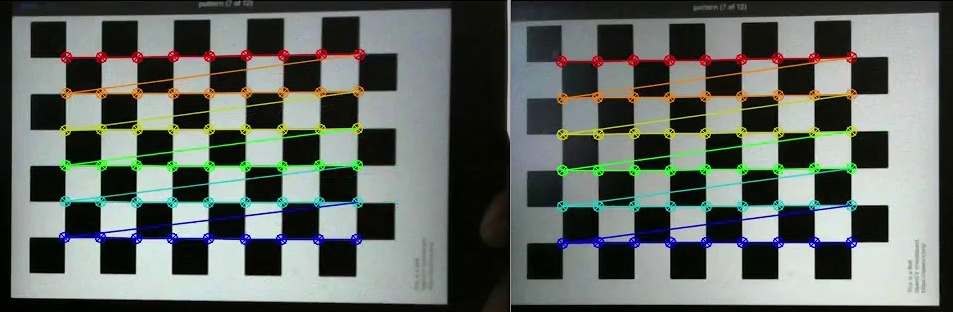
\includegraphics[width=0.8\textwidth]{images/calib.png}  % Adjust the path and width as necessary
    \captionsetup{font=footnotesize}
    \caption[Widok wykrytych wierzchołków szachownic. https://learnopencv.com/making-a-low-cost-stereo-camera-using-opencv/.]{Widok wykrytych wierzchołków szachownic.}
\end{figure}

Po wykryciu narożników ich pozycje są precyzowane za pomocą funkcji \texttt{cv2.cornerSubPix()}, co pozwala uzyskać większą dokładność w procesie kalibracji. Dane te są następnie zapisywane w postaci trzech wektorów:

\begin{itemize}
  \item imgpointsR: zawiera współrzędne narożników na prawym obrazie (w przestrzeni obrazu)
  \item imgpointsL: zawiera współrzędne narożników na lewym obrazie (w przestrzeni obrazu)
  \item objpoints: zawiera współrzędne narożników w przestrzeni obiektu.
\end{itemize}

Dane te wykorzystywane są przez funkcję \texttt{cv2.calibrateCamera()} do wyznaczenia macierzy kamery, współczynników dystorsji oraz wektorów rotacji i translacji dla każdej kamery. Macierz wewnętrzna kamery $\mathbf{M}$ opisuje rzutowanie punktów ze świata 3D na obraz 2D i przyjmuje postać:

\[
\mathbf{M} =
\begin{bmatrix}
f_x & 0 & c_x \\
0 & f_y & c_y \\
0 & 0 & 1
\end{bmatrix}
\]

\begin{itemize}
  \item $f_x = f \cdot s_x$ — ogniskowa wyrażona w pikselach w poziomie (oś X)
  \item $f_y = f \cdot s_y$ — ogniskowa wyrażona w pikselach w pionie (oś Y)
  \item $c_x$, $c_y$ — współrzędne punktu głównego (\textit{principal point}), zazwyczaj w centrum obrazu
  \item Zera poza przekątną oznaczają brak nachylenia między osiami (czyli brak efektu trapezowego)
  \item Wartość $1$ w prawym dolnym rogu służy do zapewnienia jednorodności w transformacjach macierzowych
\end{itemize}

Przykładowe macierze kamer lewej i prawej uzyskane po kalibracji przedstawiają się następująco:

\[
\mathbf{M}_L =
\begin{bmatrix}
777,7 & 0 & 345,1 \\
0 & 780,6 & 171,3 \\
0 & 0 & 1 \\
\end{bmatrix}
\qquad
\mathbf{M}_R =
\begin{bmatrix}
792,2 & 0 & 274,9 \\
0 & 801,4 & 212,9 \\
0 & 0 & 1 \\
\end{bmatrix}
\]

W celu dalszego przetwarzania obrazów i uzyskania lepszej dokładności, macierze te mogą zostać zoptymalizowane przy użyciu funkcji cv2.getOptimalNewCameraMatrix(). Zoptymalizowane wersje macierzy, uwzględniające rzeczywisty obszar widzenia i dystorsje, są wykorzystywane podczas rektyfikacji obrazów za pomocą funkcji cv2.stereoRectify().

\[
\mathbf{M}_L =
\begin{bmatrix}
636,0 & 0 & 399,6 \\
0 & 760,1 & 170,2 \\
0 & 0 & 1 \\
\end{bmatrix}
\qquad
\mathbf{M}_R =
\begin{bmatrix}
772,2 & 0 & 284,1 \\
0 & 755,5 & 217,8 \\
0 & 0 & 1 \\
\end{bmatrix}
\]

Aby wyznaczyć wzajemne położenie kamer względem siebie (rotację i translację), wykorzystywana jest funkcja cv2.stereoCalibrate(), która pozwala określić pełną konfigurację geometryczną układu stereo. Parametry te są niezbędne do poprawnego przekształcenia obrazów oraz dalszej analizy głębi, np. przy obliczaniu mapy dysparycji.

\section{Rektyfikacja stereo}

Jednym z kluczowych zagadnień w stereowizji jest \textbf{geometria epipolarna}, która opisuje zależność pomiędzy rzutami punktów przestrzennych na dwa obrazy uzyskane z różnych punktów widzenia. Celem tej geometrii jest ograniczenie przestrzeni poszukiwania punktów odpowiadających w drugim obrazie, co znacząco upraszcza dopasowywanie i rekonstrukcję głębi.

Aby dodatkowo uprościć ten proces, stosuje się \textbf{rektyfikację stereo}, czyli transformację obrazów, która sprowadza linie epipolarne do postaci równoległych i poziomych. Dzięki temu dopasowywanie punktów może być wykonywane wzdłuż jednej osi (najczęściej poziomej), co przyspiesza obliczenia i zwiększa ich dokładność.

\subsection{Geometria epipolarna}

\begin{figure}[H]
    \centering
    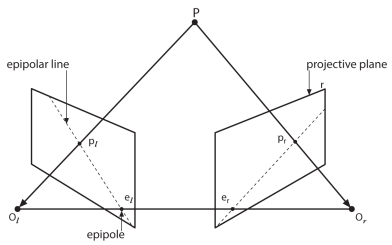
\includegraphics[width=0.5\textwidth]{images/epipolar.png}
    \captionsetup{font=footnotesize}
    \caption[Model kamery stereo. Learning OpenCV 3, O'Reilly, Str. 709]{Model kamery stereo.}
    \label{fig:rpi}
\end{figure}

Na rysunku \ref{fig:rpi} przedstawiono uproszczony model kamery stereo zbudowanej z dwóch kamer otworkowych. Punkty $O_l$ i $O_r$ to środki rzutów lewej i prawej kamery. Proste łączące punkty $p_l$ z $e_l$ oraz $p_r$ z $e_r$ to tzw. \textbf{linie epipolarne}, natomiast punkty $e_l$ i $e_r$ to \textbf{epipole} – rzuty środka jednej kamery na płaszczyznę obrazu drugiej.

Geometria epipolarna umożliwia ograniczenie przestrzeni przeszukiwania punktu odpowiadającego z pełnej płaszczyzny obrazu do jednej linii – linii epipolarnej. Ułatwia to znacznie proces dopasowywania punktów. Można to podsumować w następujących punktach:

\begin{itemize}
    \item Każdy punkt przestrzenny należy do płaszczyzny epipolarnej.
    \item Odpowiadający mu punkt w drugim obrazie musi leżeć na odpowiedniej linii epipolarnej (warunek epipolarny).
    \item Proces wyszukiwania punktu korespondującego można zredukować do jednego wymiaru, jeżeli znana jest geometria epipolarna.
    \item Kolejność punktów na liniach epipolarnych jest zachowana między obrazami.
\end{itemize}

\subsection{Macierz fundamentalna i esencjalna}

Aby matematycznie opisać zależności pomiędzy punktami w dwóch obrazach, wykorzystuje się dwie macierze: \textbf{macierz esencjalną} $E$ oraz \textbf{macierz fundamentalną} $F$. Macierz $E$ opisuje wzajemną orientację kamer (rotację i translację), natomiast $F$ uwzględnia dodatkowo parametry wewnętrzne kamer, takie jak ogniskowa czy środek obrazu.

Związek pomiędzy punktami $p_l$ i $p_r$ w obrazach opisuje równanie epipolarne:
\[
p_r^T E p_l = 0
\]

Ponieważ macierz $E$ ma rangę 2, opisuje ona jedynie płaszczyznę, nie zaś pełną transformację punktów. Dlatego wprowadza się macierz $F$, którą oblicza się jako:
\[
F = (M_r^{-1})^T E M_l^{-1}
\]
gdzie $M_l$ i $M_r$ to macierze wewnętrzne lewej i prawej kamery, a $q = M p$ to przekształcenie punktu przestrzennego do przestrzeni obrazu. Zatem pełna forma równania epipolarnego to:
\[
q_r^T F q_l = 0
\]

\subsection{Macierz obrotu i wektor translacji}

Aby wyznaczyć relację przestrzenną między kamerami, definiuje się:

\begin{itemize}
    \item $P_l = R_l P + T_l$ – przekształcenie punktu przestrzennego $P$ do układu lewej kamery,
    \item $P_r = R_r P + T_r$ – analogiczne przekształcenie do układu prawej kamery.
\end{itemize}

Na tej podstawie można wyznaczyć:
\[
P_l = R(P_r - T)
\]

co prowadzi do zależności:
\[
R = R_r R_l^T, \quad T = T_r - R T_l
\]

\subsection{Algorytmy rektyfikacji w OpenCV}

Celem rektyfikacji jest takie przekształcenie obrazów, aby ich linie epipolarne były współliniowe i poziome. W praktyce oznacza to sprowadzenie układów optycznych obu kamer do tej samej płaszczyzny rzutowania.

W wyniku rektyfikacji uzyskuje się dla każdej kamery:

\begin{itemize}
    \item wektor dystorsji,
    \item macierz rotacji rektyfikującej $R_{\text{rect}}$,
    \item zrektyfikowaną macierz projekcji $M_{\text{rect}}$,
    \item oryginalną (niezrektyfikowaną) macierz kamery $M$.
\end{itemize}

\subsection*{Algorytm Hartley’a}

Algorytm Hartley’a \cite{hartley} pozwala przeprowadzić rektyfikację obrazów bez znajomości parametrów wewnętrznych kamer (metoda niekalibrowana).

\textbf{Etapy działania:}
\begin{itemize}
    \item Wyszukiwanie punktów korespondencyjnych (np. z użyciem cech SIFT, SURF, ORB),
    \item Estymacja macierzy fundamentalnej $F$,
    \item Obliczenie homografii, które przekształcają epipole do nieskończoności (linie epipolarne stają się poziome).
\end{itemize}

Wadą tej metody jest brak informacji o rzeczywistej skali sceny – relacje przestrzenne są wyłącznie względne.

\noindent Przykładowa implementacja w Pythonie z wykorzystaniem funkcji \texttt{stereoRectifyUncalibrated} z biblioteki OpenCV:

\begin{lstlisting}[style=mypython]
# Wykrycie i opis cech (np. ORB)
orb = cv2.ORB_create()
kp1, des1 = orb.detectAndCompute(imgL, None)
kp2, des2 = orb.detectAndCompute(imgR, None)

# Dopasowanie cech metodą BFMatcher
bf = cv2.BFMatcher(cv2.NORM_HAMMING, crossCheck=True)
matches = bf.match(des1, des2)
matches = sorted(matches, key=lambda x: x.distance)

# Konwersja dopasowań do tablic punktów
pts1 = np.float32([kp1[m.queryIdx].pt for m in matches]).reshape(-1,1,2)
pts2 = np.float32([kp2[m.trainIdx].pt for m in matches]).reshape(-1,1,2)

# Estymacja macierzy fundamentalnej
F, mask = cv2.findFundamentalMat(pts1, pts2, cv2.FM_RANSAC)

# Wybór tylko inlierów
pts1 = pts1[mask.ravel()==1]
pts2 = pts2[mask.ravel()==1]

# Obliczenie homografii rektyfikujących
ret, H1, H2 = cv2.stereoRectifyUncalibrated(
    pts1, pts2, F, imgSize=imgL.shape[::-1]
)

# Zastosowanie przekształceń homograficznych
imgL_rect = cv2.warpPerspective(imgL, H1, imgL.shape[::-1])
imgR_rect = cv2.warpPerspective(imgR, H2, imgR.shape[::-1])
\end{lstlisting}

\subsection*{Algorytm Bouguet’a}

Algorytm Bouguet’a \cite{bouget}, stosowany m.in. w narzędziu \textit{Camera Calibration Toolbox} dla MATLAB-a, opiera się na wcześniejszej kalibracji kamer (metoda kalibrowana).

\textbf{Etapy działania:}
\begin{itemize}
    \item Kalibracja kamer z wykorzystaniem wzorca (np. szachownicy),
    \item Wyznaczenie parametrów wewnętrznych i zewnętrznych (R i T),
    \item Przekształcenie obrazów tak, aby ich osie optyczne były równoległe,
    \item Wygenerowanie zrektyfikowanych obrazów, w których odpowiadające piksele leżą na tych samych liniach poziomych.
\end{itemize}

Metoda ta zapewnia większą precyzję, lecz jest wrażliwa na błędy kalibracji (np. niedokładne wykrycie wzorca).

\begin{lstlisting}[style=mypython]
# Funkcja stereoRectify
RL, RR, PL, PR, Q, roiL, roiR = cv2.stereoRectify(MLS, dLS, MRS, dRS,
                                              ChessImgR.shape[::-1], R, T, 0, (0, 0))
# Generowanie map przekształceń
Left_Stereo_Map = cv2.initUndistortRectifyMap(MLS, dLS, RL, PL,
                                              ChessImgR.shape[::-1], cv2.CV_16SC2)
Right_Stereo_Map = cv2.initUndistortRectifyMap(MRS, dRS, RR, PR,
                                              ChessImgR.shape[::-1], cv2.CV_16SC2)
\end{lstlisting}

Funkcja \texttt{cv2.stereoRectify()} przekształca obrazy w taki sposób, aby ich linie epipolarne były poziome. Z kolei \texttt{cv2.initUndistortRectifyMap()} umożliwia wygenerowanie obrazów bez dystorsji i z poprawną geometrią epipolarną.

\textbf{Przykładowe macierze kalibracyjne:}

\[
\mathbf{M}_L =
\begin{bmatrix}
791.0 & 0 & 390.6 \\
0 & 791.0 & 194.4 \\
0 & 0 & 1 \\
\end{bmatrix}
\qquad
\mathbf{M}_R =
\begin{bmatrix}
791.0 & 0 & 390.6 \\
0 & 791.0 & 194.4 \\
0 & 0 & 1 \\
\end{bmatrix}
\]

Tak przygotowane obrazy mogą być bezpośrednio wykorzystane do obliczania mapy dysparycji oraz rekonstrukcji 3D.

\section{Mapa dysparycji}

Mapa dysparycji\cite{disparity} to obraz, w którym każdemu pikselowi przypisywana jest wartość reprezentująca przesunięcie (różnicę pozycji) pomiędzy odpowiadającymi sobie punktami w obrazie lewym i prawym. Im większe przesunięcie (czyli dysparycja), tym bliżej znajduje się dany obiekt względem kamery. Taka mapa stanowi podstawę do obliczenia mapy głębokości, która pozwala oszacować odległość poszczególnych punktów sceny od obserwatora.

\subsection*{Algorytm StereoSGBM}

\begin{lstlisting}[style=mypython]
# Inicjalizacja StereoSGBM
block_size = 7
min_disp = 2
num_disp = 130-min_disp
stereo = cv2.StereoSGBM_create(
    minDisparity = min_disp,
    # Minimalna dysparycja (najmniejsze oczekiwane przesunięcie pikseli).
    # Zwykle 0 lub lekko dodatnia wartość, jeśli obiekty mogą być bardzo daleko.
    numDisparities = num_disp,
    # Liczba możliwych poziomów dysparycji (musi być podzielna przez 16!).
    # Określa zakres przeszukiwania. Większy = można wykryć bliższe obiekty.
    blockSize = block_size,
    # Rozmiar bloku dopasowania (okno porównywane między obrazami).
    # Większe wartości = lepsza odporność na szumy, ale gorsza precyzja brzegów.
    uniquenessRatio = 10,
    # Minimalna różnica procentowa między najlepszym a drugim najlepszym dopasowaniem.
    # Pomaga odrzucać niepewne wyniki - im wyższa wartość, tym ostrzejsze kryterium.
    speckleWindowSize = 100,
    # Maksymalny rozmiar obszaru z "plamkami" (ang. speckles), który zostanie usunięty.
    # Używane do usuwania małych, niespójnych obszarów w mapie dysparycji.
    speckleRange = 32,
    # Maksymalna dozwolona różnica dysparycji w obrębie speckle.
    # Pomaga wyciąć obszary o nietypowych skokach dysparycji.
    disp12MaxDiff = 5,
    # Maksymalna dopuszczalna różnica między wynikami z dopasowania lewo-prawo i prawo-lewo.
    # Służy do sprawdzania spójności dopasowania - niskie wartości odrzucają więcej niepewnych pikseli.
    P1 = 8*3*block_size**2,
    # Kara za niewielkie zmiany dysparycji między sąsiednimi pikselami (gładkość).
    # Wzór zależy od liczby kanałów (3 dla koloru) i wielkości bloku.
    P2 = 32*3*block_size**2
    # Kara za większe zmiany dysparycji (duże skoki).
    # Powinna być większa niż P1 - większe wartości = bardziej gładka mapa dysparycji.
)

# Tworzy druga instancje StereoSGBM, identyczna jak stereo,
# ale z ustawieniami odpowiednimi do przetwarzania prawego obrazu wzgledem lewego.
stereoR=cv2.ximgproc.createRightMatcher(stereo)
\end{lstlisting}

Aby obliczyć mapę dysparycji, wykorzystywany jest obiekt klasy StereoSGBM, tworzony za pomocą funkcji \texttt{cv2.StereoSGBM-create()}. Algorytm ten wykorzustuje metodę półglobalnego dopasowania blokowego (ang. \textit{Semi-Global Block Matching}) \cite{semi-global}, która umożliwia estymację przesunięć pomiędzy obrazami stereo — z lewej i prawej kamery.

Jednym z kluczowych parametrów wejściowych algorytmu jest rozmiar bloku, który określa wielkość lokalnego sąsiedztwa wykorzystywanego do dopasowania. W przypadku, gdy wartość ta jest większa niż 1, algorytm operuje nie na pojedynczych pikselach, lecz na blokach. W praktyce oznacza to, że każdy blok z obrazu referencyjnego (np. lewego) porównywany jest z blokami z obrazu dopasowywanego (np. prawego) w celu znalezienia najlepszego dopasowania.

Jeśli stereo-kalibracja i rektyfikacja zostały przeprowadzone poprawnie, porównania odbywają się jedynie wzdłuż odpowiadających sobie wierszy, czyli linii epipolarnych. Dzięki temu przeszukiwanie ogranicza się do jednej wymiarowej przestrzeni (poziomej), co znacznie zmniejsza złożoność obliczeniową algorytmu.

Na przykład, blok o współrzędnych (4,7) w obrazie bazowym zostaje porównany z wszystkimi blokami (4, i) w tej samej linii epipolarnej obrazu dopasowywanego.

\begin{figure}[H]
\centering
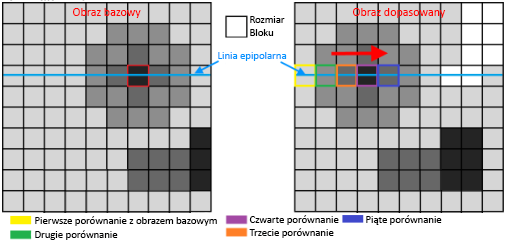
\includegraphics[width=0.8\textwidth]{images/dopracy1.png}
\captionsetup{font=footnotesize}
\caption[Wyszukiwanie pasujących bloków za pomocą StereoSGBM. Opracowanie własne.]{Wyszukiwanie pasujących bloków za pomocą StereoSGBM.}
\end{figure}

Im większy stopień dopasowania między blokami, tym większe prawdopodobieństwo, że reprezentują one ten sam punkt w przestrzeni trójwymiarowej. W przedstawionym przykładzie najwyższe dopasowanie dla bloku referencyjnego (4,7) uzyskano względem bloku (4,4) w obrazie dopasowywanym.

Choć w teorii dopasowania dokonuje się tylko w jednym kierunku (poziomym), implementacja algorytmu w OpenCV zakłada analizę także w dodatkowych kierunkach (łącznie pięciu), co pozwala na zwiększenie dokładności dopasowań poprzez uwzględnienie lokalnych kontekstów z różnych stron.

\begin{figure}[H]
\centering
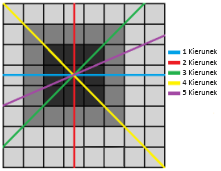
\includegraphics[width=0.5\textwidth]{images/dopracy2.png}
\captionsetup{font=footnotesize}
\caption[Pięć kierunków przeszukiwania w algorytmie StereoSGBM. Opracowanie własne.]{Pięć kierunków przeszukiwania w algorytmie StereoSGBM.}
\end{figure}

Wartość dysparycji uzyskuje się poprzez obliczenie różnicy poziomej współrzędnej piksela (lub bloku) w obrazie referencyjnym i odpowiadającej mu pozycji w obrazie dopasowywanym. W praktyce przyjmuje się wartość bezwzględną tej różnicy, a im jest ona większa, tym obiekt znajduje się bliżej kamery (zgodnie z zasadą triangulacji w stereowizji).

Algorytm zazwyczaj operuje na obrazach w odcieniach szarości (jednokanałowych), co pozwala znacząco zredukować czas obliczeń. Możliwe jest również zastosowanie obrazów kolorowych (np. w przestrzeni BGR), jednak wiąże się to ze zwiększonym obciążeniem procesora, bez gwarancji proporcjonalnej poprawy wyników.

Właściwa mapa dysparycji obliczana jest przy użyciu metody \texttt{compute()} na wcześniej skonfigurowanym obiekcie StereoSGBM.

Dzięki parametrom ustalonym podczas inicjalizacji otrzymujemy następujący wynik dla mapy dysparycji.

\begin{figure}[H]  % 'h' means "here", it places the figure at the current location in the document
    \centering  % Centers the image
    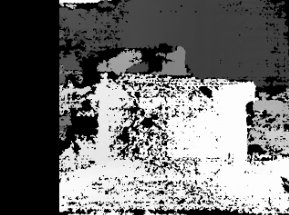
\includegraphics[width=0.4\textwidth]{images/dopracy3.png}  % Adjust the path and width as necessary
    \captionsetup{font=footnotesize}
    \caption[Wynik dla mapy dysproporcji. Opracowanie własne.]{Wynik dla mapy dysproporcji.}
\end{figure}

Na wygenerowanej mapie dysparycji mogą nadal występować zakłócenia w postaci lokalnych szumów. W celu ich redukcji stosuje się filtrację morfologiczną, która pozwala poprawić spójność i ciągłość danych głębokości. W szczególności wykorzystywany jest operator zamykania (morphological closing), realizowany w OpenCV za pomocą funkcji \texttt{cv2.morphologyEx()} z flagą \texttt{cv2.MORPH\_CLOSE}. Zastosowanie tego filtru pozwala na eliminację drobnych czarnych artefaktów, które mogą pojawić się wewnątrz jednorodnych obszarów na mapie.

\begin{figure}[H]  % 'h' means "here", it places the figure at the current location in the document
    \centering  % Centers the image
    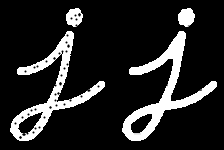
\includegraphics[width=0.4\textwidth]{images/closing.png}  % Adjust the path and width as necessary
    \captionsetup{font=footnotesize}
    \caption[Przykład filtra zamykającego. https://docs.opencv.org/3.4/d9/d61/tutorial-py-morphological-ops.html]{Przykład filtra zamykającego.}
\end{figure}

Poniżej inny przykład tej samej sceny, aby lepiej zobaczyć różnicę.

\begin{figure}[H]  % 'h' means "here", it places the figure at the current location in the document
    \centering  % Centers the image
    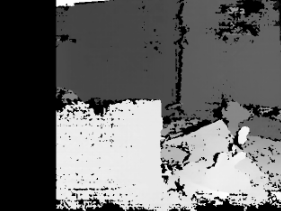
\includegraphics[width=0.4\textwidth]{images/dopracy4.png}  % Adjust the path and width as necessary
    \captionsetup{font=footnotesize}
    \caption[Wynik mapy dysproporcji po filtrze zamykającym. Opracowanie własne.]{Wynik mapy dysproporcji po filtrze zamykającym.}
\end{figure}

\subsection*{Algorytm StereoBM}

Alternatywą dla metody \texttt{StereoSGBM} jest \texttt{StereoBM} (ang. \textit{Block Matching}) \cite{bm}, będący jedną z najstarszych implementacji dopasowania stereoskopowego w bibliotece OpenCV. Algorytm ten bazuje na bezpośrednim porównywaniu bloków pikseli pomiędzy obrazem lewym i prawym wzdłuż linii epipolarnych, wykorzystując prostą funkcję kosztu, np. \textit{Sum of Absolute Differences} (SAD).

Inicjalizacja przebiega następująco:

\begin{lstlisting}[style=mypython]

Inicjalizacja StereoBM
num_disp = 64 # musi być podzielne przez 16
block_size = 15 # większy blok = większa odporność na szumy

stereo_bm = cv2.StereoBM_create(
numDisparities=num_disp,
blockSize=block_size
)

Obliczenie mapy dysparycji
disparity_bm = stereo_bm.compute(grayL, grayR)
\end{lstlisting}

W odróżnieniu od \texttt{StereoSGBM}, algorytm \texttt{StereoBM} analizuje jedynie lokalne dopasowania bez optymalizacji globalnej. Dzięki temu jest znacząco szybszy i mniej zasobożerny, co czyni go dobrym wyborem w systemach wbudowanych (np. Raspberry~Pi) lub w aplikacjach wymagających przetwarzania w czasie rzeczywistym. Jednak jego prostota powoduje większą wrażliwość na szumy i mniejszą dokładność w obszarach jednorodnych lub przy słabym tekście.

Podobnie jak w przypadku \texttt{StereoSGBM}, poprawna rektyfikacja obrazów jest warunkiem uzyskania wiarygodnej mapy dysparycji. Ze względu jednak na mniejszą złożoność obliczeń, \texttt{StereoBM} wymaga często dodatkowych filtrów (np. medianowego lub morfologicznego) w celu poprawy jakości wyników.

\section{Filtr WLS}

\begin{lstlisting}[style=mypython]
# Parametry filtra WLS
wls_filter = cv2.ximgproc.createDisparityWLSFilter(matcher_left=stereo)
wls_filter.setLambda(80000)
wls_filter.setSigmaColor(1.8)
\end{lstlisting}

W celu dalszego ograniczenia szumu w mapie dysparycji stosowany jest filtr ważonych najmniejszych kwadratów(ang. \textit{Weighted Least Squares}) \cite{wls}, dostępny w module \texttt{cv2.ximgproc}. Jest on szczególnie skuteczny w poprawianiu ciągłości strukturalnej oraz w zachowaniu ostrych krawędzi w scenach o złożonej geometrii.

Parametr lambda kontroluje stopień wygładzania mapy: im wyższa jego wartość, tym bardziej struktura wynikowej mapy przypomina obraz referencyjny (np. lewy obraz stereo). W praktyce często stosuje się wartości rzędu 8000, jednak w omawianym przypadku zastosowano wartość \texttt{lambda = 80000}, co pozwoliło uzyskać bardziej stabilne rezultaty. Z kolei parametr sigma określa, jak precyzyjnie filtr ma traktować obszary znajdujące się w pobliżu krawędzi – wyższe wartości sprzyjają lepszemu zachowaniu konturów obiektów.

Aby skorzystać z filtra WLS, tworzony jest dodatkowy obiekt dopasowania stereo dla prawego obrazu, przy użyciu funkcji \texttt{cv2.ximgproc.createRightMatcher()}, bazujący na głównym obiekcie StereoSGBM. Następnie inicjalizowany jest filtr WLS poprzez \texttt{cv2.ximgproc.\allowbreak createDisparityWLSFilter()} i konfigurowany z użyciem uprzednio utworzonych dopasowań.

Sam proces filtracji przeprowadzany jest metodą \texttt{filter()} filtra WLS, a jego wynik poddawany jest normalizacji za pomocą funkcji \texttt{cv2.normalize()}, co pozwala na wizualizację rezultatu.

Należy jednak zauważyć, że wynik filtru WLS nie jest już bezpośrednio wykorzystywalną mapą dysparycji — jest to obraz zakodowany w formacie uint8, który dobrze uwidacznia krawędzie, lecz nie zawiera już rzeczywistych wartości głębokości (w przeciwieństwie do oryginalnej mapy dysparycji w formacie float32).

\section{Główna pętla}

\begin{lstlisting}[style=mypython]
while True:

    ret, frame = Cam.read()
    if not ret:
        # Przerwij jesli nie odczytano klatki z kamery
        break

    height, width, _ = frame.shape
    mid = width // 2

    left_frame = executor.submit(lambda: frame[:, :mid])
    right_frame = executor.submit(lambda: frame[:, mid:])
    LFrame = left_frame.result()
    RFrame = right_frame.result()

    # Rownolegle operacje remapowania 
    future_Left_nice = executor.submit(cv2.remap, LFrame,
                                Left_Stereo_Map[0], Left_Stereo_Map[1],
                                interpolation=cv2.INTER_LANCZOS4,
                                borderMode=cv2.BORDER_CONSTANT)
    future_Right_nice = executor.submit(cv2.remap, RFrame,
                                Right_Stereo_Map[0], Right_Stereo_Map[1],
                                interpolation=cv2.INTER_LANCZOS4,
                                borderMode=cv2.BORDER_CONSTANT)
    Left_nice = future_Left_nice.result()
    Right_nice = future_Right_nice.result()

    # Rownolegla konwersja na skale szarosci
    future_gray_left = executor.submit(cv2.cvtColor, Left_nice, cv2.COLOR_BGR2GRAY)
    future_gray_right = executor.submit(cv2.cvtColor, Right_nice, cv2.COLOR_BGR2GRAY)
    Gray_left = future_gray_left.result()
    Gray_right = future_gray_right.result()

    # Rownolegla kalkukacja dysproporcji
    future_dispL = executor.submit(stereo.compute, Gray_left, Gray_right)
    future_dispR = executor.submit(stereoR.compute, Gray_right, Gray_left)
    DispL = np.int16(future_dispL.result())
    DispR = np.int16(future_dispR.result())

    disp = ((DispL.astype(np.float32) / 16) - min_disp) / num_disp

    filteredImg = wls_filter.filter(DispL, Gray_left, None, DispR)
    filteredImg = cv2.normalize(src=filteredImg, dst=filteredImg, beta=0, 
                                alpha=255, norm_type=cv2.NORM_MINMAX)
    filteredImg = np.uint8(filteredImg)

    filt_Color = cv2.applyColorMap(filteredImg, cv2.COLORMAP_OCEAN)
\end{lstlisting}

Po wygenerowaniu mapy dysparycji należy określić odległość. Zadanie polega na znalezieniu zależności między wartością dysparycji, a odległością. Aby to zrobić, eksperymentalnie zmierzyliśmy wartości dysparycji w kilku miejscach, aby na tej podstawie określić regresję.

\begin{lstlisting}[style=mypython]
_, close_mask = cv2.threshold(filteredImg, 160, 255, cv2.THRESH_BINARY)
close_mask = cv2.morphologyEx(close_mask, cv2.MORPH_CLOSE, kernel)
contours, _ = cv2.findContours(close_mask, cv2.RETR_EXTERNAL, cv2.CHAIN_APPROX_SIMPLE)

for cnt in contours:
    if cv2.contourArea(cnt) > 500:
        x, y, w, h = cv2.boundingRect(cnt)

        roi_disp = disp[y:y + h, x:x + w].astype(np.float32)
        cx, cy = x + w // 2, y + h // 2
        sample_disp = disp[cy - 1:cy + 2, cx - 1:cx + 2].astype(np.float32)
        average_disp = np.mean(sample_disp[sample_disp > 0])

        if average_disp > 0:
            distance = -593.97 * average_disp**3 + 1506.8 
                               * average_disp**2 - 1373.1 
                               * average_disp + 522.06
            distance = np.around(distance * 0.01, decimals=2)

            if distance < 1.0:
                box_color = (0, 0, 255) if distance < 0.5 else (0, 255, 0)
                cv2.rectangle(filt_Color, (x, y), (x + w, y + h), box_color, 2)
                cv2.putText(filt_Color, f"{distance:.2f} m", (x, y - 10),
                            cv2.FONT_HERSHEY_SIMPLEX, 0.5, box_color, 2)
\end{lstlisting}

Obraz filteredImg (np. przefiltrowany obraz po detekcji koloru lub kształtu) jest zamieniany na obraz czarno-biały (binary mask), gdzie tylko jasne piksele > 160 zostają. Następnie nakłada się na ten obraz filtr domknięcia (closing).

Funkcja findContours wykrywa obiekty (kontury) w masce. RETR\_EXTERNAL oznacza, że interesują nas tylko zewnętrzne kontury.

Pętla sprawdza każdy kontur. Kontury mniejsze niż 500 pikseli są ignorowane (eliminacja szumów).

Z mapy dysparycji obliczany jest bounding box wokół konturu, następnie wycinany jest fragment mapy dysparycji w tym obszarze. Z jego środka (cx, cy) pobierany jest mały fragment (3×3) do analizy.

Obliczana jest średnia dysparycja. Z 3×3 pikseli ze środka wybierane są tylko te z sensowną wartością (większą od zera).

Na podstawie średniej dysparycji obliczana jest odległość w metrach. Użyty jest wzór aproksymacyjny (polinom).

Wynik skalowany jest do metrów i zaokrąglany do 2 miejsc po przecinku.

Jeśli obiekt znajduje się bliżej niż 1 metr, rysowana jest prostokątna ramka: czerwona jeśli < 0.5 m, zielona jeśli 0.5 – 1.0 m.

Nad obiektem wyświetlana jest informacja o odległości w metrach.

Pomiar odległości dotyczy tylko odległości od 67 cm do 203 cm, aby uzyskać dobre wyniki. Precyzja pomiaru zależy również od jakości kalibracji. Kamera stereo były w stanie zmierzyć odległość do obiektu z precyzją ± 5 cm.

Zwrócona wartość to średnia dysparycji z macierzy 9x9 pikseli.

\section{Triangulacja}

\begin{figure}[H]  % 'h' means "here", it places the figure at the current location in the document
    \centering  % Centers the image
    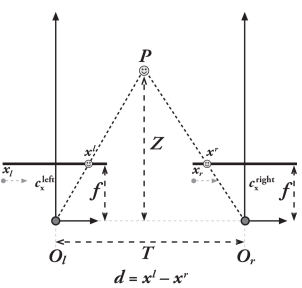
\includegraphics[width=0.5\textwidth]{images/triangulation.png}  % Adjust the path and width as necessary
    \captionsetup{font=footnotesize}
    \caption[Schemat triangulacji. Learning OpenCV 3, O'Reilly, Str. 705]{Schemat triangulacji.}
    \label{fig:rpi}  % Optional: use to refer to this image later in the text
\end{figure}

W ostatnim kroku, triangulacji, zakłada się, że oba obrazy projekcji są współpłaszczyznowe i że poziomy rząd pikseli lewego obrazu jest wyrównany z odpowiadającym mu obrazem prawego.

Poniższy obraz można teraz skonstruować przy użyciu poprzednich hipotez.

Punkt $P$ leży w środowisku i jest pokazany na
lewym i prawym obrazie na $P_l$ i $P_r$, z odpowiadającymi im współrzędnymi
odpowiadającymi współrzędnymi $X_l$ i $X_r$. To pozwala nam wprowadzić nową wielkość $d = X_l - X_r$.
Można zauważyć, że im dalej punkt $P$, tym mniejsza staje się wielkość $d$. Dysproporcja jest zatem odwrotnie proporcjonalna do odległości.\\
Do obliczenia odległości można użyć następującego wzoru można obliczyć: \[Z=f*T/(xl-xr)\]

Można zauważyć, że istnieje nieliniowa zależność między rozbieżnością a odległością.
Jeśli rozbieżność jest bliska 0, małe różnice w rozbieżności prowadzą do dużych różnic w odległości.
Zjawisko to ulega odwróceniu, gdy rozbieżność jest duża. Małe różnice dysproporcji nie prowadzą do dużych różnic odległości. Na tej podstawie można wywnioskować, że stereowizja ma wysoką rozdzielczość głębi, tylko dla obiektów znajdujących się blisko kamery.

Metoda ta działa jednak tylko wtedy, gdy konfiguracja kamery stereo jest idealna. W
rzeczywistości tak nie jest. Właśnie dlatego lewy i prawy obraz są
matematycznie wyrównane równolegle. Oczywiście kamery muszą być fizycznie ustawione równolegle.
Zanim zostanie wyjaśniona metoda matematycznego wyrównywania obrazów, trzeba najpierw zrozumieć geometrię epipolarną.

\section{Wnioski i możliwe ulepszenia}

\begin{minipage}[t]{\textwidth}
\textbf{Wady i ograniczenia STEREO:}
\begin{itemize}
  \item Wymóg kalibracji i synchronizacji kamer – błędy w tym zakresie przekładają się bezpośrednio na błędną głębokość.

  \item Brak dopasowania w teksturowo ubogich obszarach – np. białe ściany, niebo.

  \item Problemy przy silnym oświetleniu i odbiciach – zmienność intensywności zaburza dopasowanie.

  \item Duży koszt obliczeniowy – szczególnie w przypadku metod globalnych lub opartych na deep learningu.

  \item Widzenie tylko z jednej perspektywy – martwe strefy między kamerami lub poza polem widzenia jednej z nich.
\end{itemize}
\end{minipage}

Możliwe ulepszenia dla programu:

Należy wziąć kształt filtra WLS i projektować go na mapie dysparycji. Ta projekcja zostanie następnie użyta do pobrania wszystkich wartości dysparycji, które znajdują się w tym kształcie, a wartość, która występuje najczęściej, zostanie ustawiona jako wartość dla całej powierzchni.

Użycie filtra bilateralnego na skalibrowanych obrazach przed wygenerowaniem mapy dysparycji, w ten sposób mogłoby być możliwe, aby nie stosować filtra WLS. Należy to sprawdzić, ale filtr WLS służy głównie do dobrego rozpoznawania krawędzi obiektów, być może istnieje lepsza metoda.

Aby skrócić czas obliczeń przy generowaniu mapy dysparycji, należy zmniejszyć skalibrowane obrazy za pomocą funkcji cv2.resize(cv2.INTER\_AbyREA). Należy przy tym pamiętać, że wartości macierzy esencjalnych i fundamentalnych również muszą być proporcjonalnie zmniejszone.

Generowanie mapy głębokości mogłoby również być korzystne.

Wystarczyłoby zapisać wartości macierzy z kalibracji stereo, aby móc je ponownie wykorzystać. Dużo czasu mogłoby to zaoszczędzić w trakcie inicjalizacji.

Uruchomienie programu na GPU pozwoliłoby również uzyskać gładsze obrazy, gdy kamera stereo jest w ruchu.

Używana równość prosta zawsze zwracałaby dokładną odległość do obiektu z większą precyzją i mniejszym nakładem pracy.

\subsubsection*{Structured Light}

\begin{figure}[H]  % 'h' means "here", it places the figure at the current location in the document
    \centering  % Centers the image
    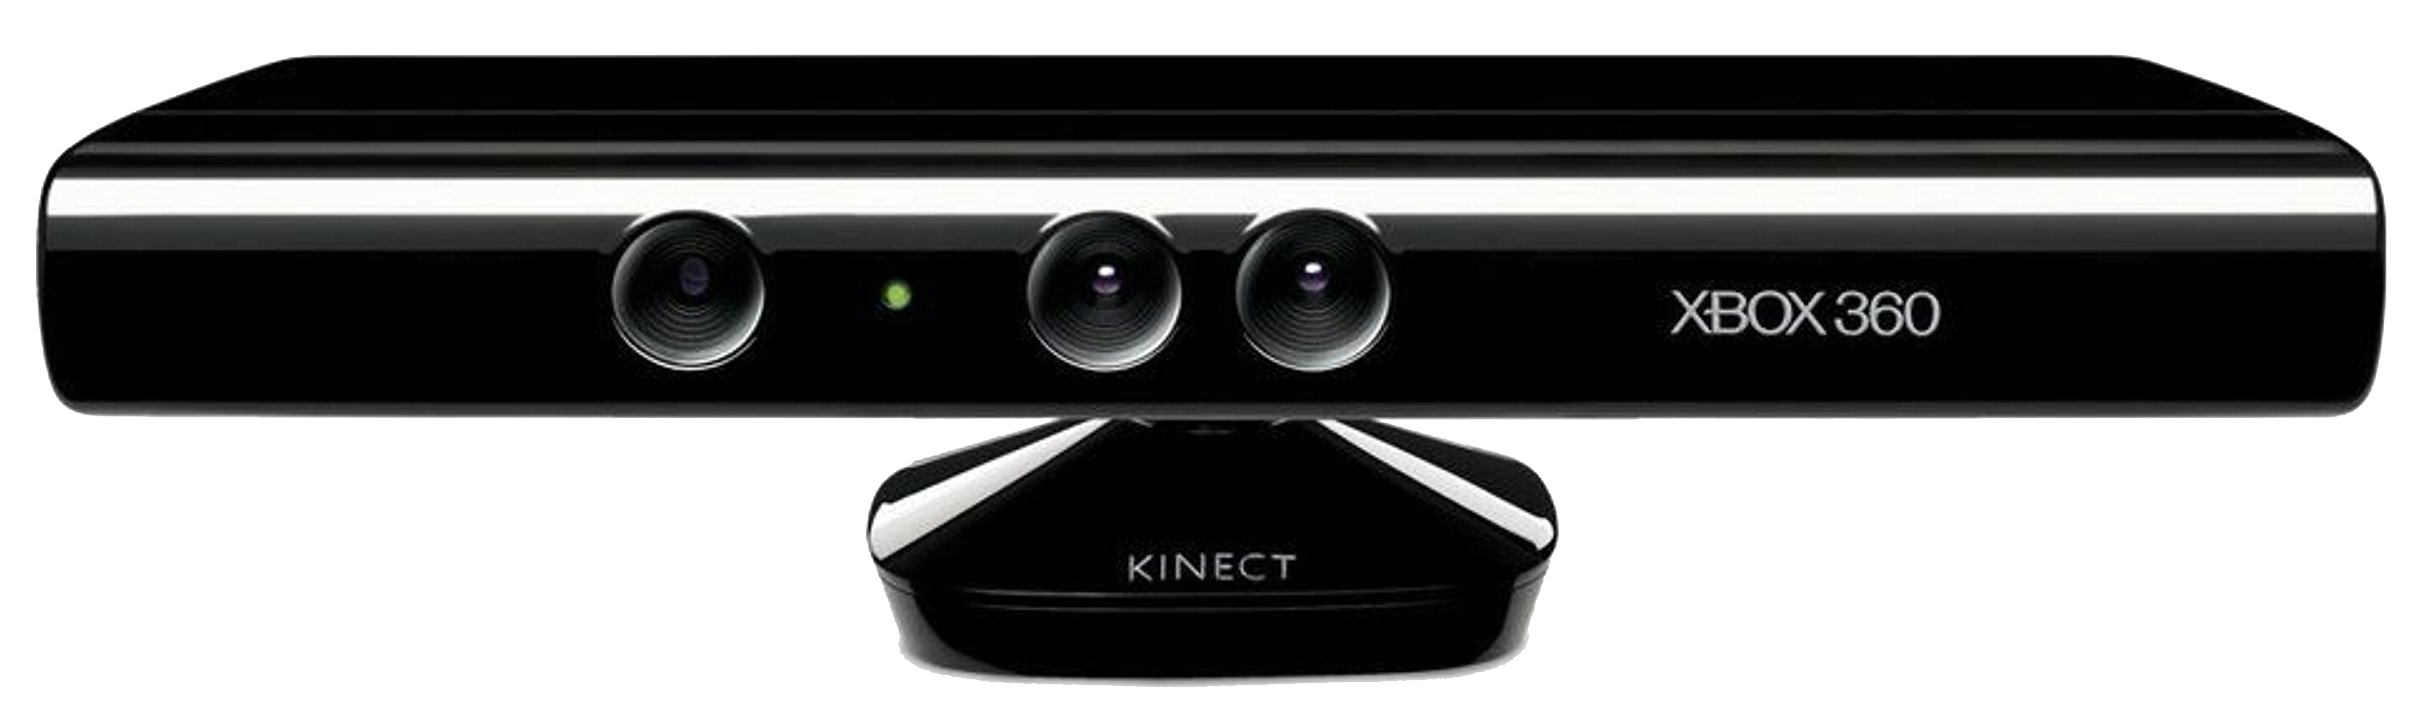
\includegraphics[width=0.5\textwidth]{images/POINTCLOUD.png}  % Adjust the path and width as necessary
    \captionsetup{font=footnotesize}
    \caption[Kamera Xbox 360 Kinect. https://cell-kom.com/inne/21454-kamera-internetowa-full-hd-b16-1080p-5900217390350.html]{Kamera Xbox 360 Kinect}
    \label{fig:kinect}  % Optional: use to refer to this image later in the text
\end{figure}

Structured Light (pol. światło strukturalne) to technika aktywnej wizji komputerowej wykorzystywana do precyzyjnego pomiaru kształtu i głębokości obiektów. Polega na projekcji znanego wzorca świetlnego (np. siatki, kropek, pasków) na powierzchnię sceny, a następnie analizie deformacji tego wzorca za pomocą kamery.

\bigskip

System Structured Light składa się zazwyczaj z dwóch komponentów:

\begin{itemize}
  \item Projektora – emituje wzorzec świetlny (np. siatkę punktów lub paski) na obserwowaną scenę.

  \item Kamery – rejestruje zniekształcony wzorzec po odbiciu od obiektów w przestrzeni.
\end{itemize}

Proces działa następująco:

\begin{enumerate}
  \item Znany wzorzec zostaje wyświetlony na scenie.

  \item Gdy wzorzec napotyka obiekty o różnych kształtach i odległościach, zostaje geometrycznie zniekształcony.

  \item Kamera rejestruje te deformacje.

  \item System porównuje zarejestrowany obraz wzorca ze wzorcem referencyjnym, który byłby widoczny na płaskiej powierzchni.

  \item Na podstawie różnic (tzw. disparity) obliczana jest głębokość – za pomocą triangulacji.
\end{enumerate}

\begin{minipage}[t]{\textwidth}
\textbf{Wady i ograniczenia:}
\begin{itemize}
  \item W jasnym świetle dziennym (szczególnie na zewnątrz), wzorzec świetlny może zostać zaburzony lub całkowicie zaniknąć – szczególnie jeśli działa w paśmie IR.

  \item Technika najlepiej sprawdza się na krótkich dystansach (0,5–2 m). Dalsze obiekty dają mniej wyraźne zniekształcenia wzorca.

  \item Szkło, lustra, woda lub powierzchnie metaliczne mogą zaburzyć wzorzec lub wprowadzać wielokrotne odbicia.

  \item Projektor i kamera muszą być precyzyjnie skalibrowane względem siebie – błędy kalibracji mogą znacząco wpłynąć na jakość głębi.

  \item Gdy wzorzec nie dotrze do części sceny (np. w załomach, pod kątem), pomiar głębokości w tych miejscach będzie niemożliwy.
\end{itemize}
\end{minipage}

\subsubsection*{LIDAR (Light Detection and Ranging)}

\begin{figure}[H]  % 'h' means "here", it places the figure at the current location in the document
    \centering  % Centers the image
    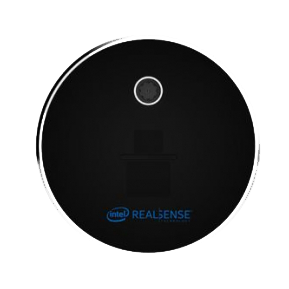
\includegraphics[width=0.3\textwidth]{images/LIDAR.png}  % Adjust the path and width as necessary
    \captionsetup{font=footnotesize}
    \caption[Kamera Intel RealSense L515 z technologią LIDAR. https://cell-kom.com/inne/21454-kamera-internetowa-full-hd-b16-1080p-5900217390350.html]{Kamera Intel RealSense z technologią LIDAR.}
    \label{fig:mono}  % Optional: use to refer to this image later in the text
\end{figure}

LIDAR (Light Detection and Ranging) to technologia zdalnego pomiaru odległości, która działa poprzez wysyłanie impulsów laserowych i mierzenie czasu, jaki upływa od ich odbicia od obiektu do powrotu do sensora. Na tej podstawie LIDAR tworzy bardzo dokładne mapy 3D otoczenia.

Podstawowy mechanizm działania LiDAR opiera się na bardzo prostej zasadzie:

\begin{itemize}
  \item Sensor emituje impuls laserowy w kierunku otoczenia.
  \item Światło odbija się od powierzchni obiektów i wraca do detektora.
  \item System mierzy czas, jaki upłynął od wysłania do odebrania sygnału (Time-of-Flight, ToF).
  \item Znając prędkość światła, obliczana jest dokładna odległość:
    \[
    d = \frac{c \cdot \Delta t}{2}
    \]

  gdzie:
  \begin{align*}
  d &- \text{odległość do obiektu} \\
  c &- \text{prędkość światła (ok. } 3 \cdot 10^8 \, \text{m/s)} \\
  \Delta t &- \text{czas przelotu sygnału}
  \end{align*} 
\end{itemize}

LiDAR-y mogą wykonywać takie pomiary miliony razy na sekundę, skanując środowisko w 2D (jeden plan) lub 3D (pełna chmura punktów).

\begin{minipage}[t]{\textwidth}
\textbf{Wady i ograniczenia:}
\begin{itemize}
  \item Mgła, deszcz, śnieg i kurz mogą zakłócać odbicie promieni lasera, co wpływa na dokładność pomiarów.

  \item Brak dopasowania w teksturowo ubogich obszarach – np. białe ściany, niebo.

  \item LiDAR rejestruje wyłącznie dane geometryczne – nie dostarcza żadnych informacji o kolorze czy teksturze powierzchni.

  \item W porównaniu do kamer, LiDAR-y mają stosunkowo rzadką siatkę pomiarową, co skutkuje niższą rozdzielczością przy dużych odległościach (np. obiekt 100 m dalej może być opisany przez kilka punktów).

  \item Bardzo ciemne lub przezroczyste powierzchnie (np. szyby) mogą słabo odbijać impulsy lasera lub w ogóle je przepuszczać.
\end{itemize}
\end{minipage}

\subsubsection*{Kamery zdarzeniowe}

Kamery zdarzeniowe (ang. Event Cameras) to innowacyjne sensory wizyjne, które różnią się fundamentalnie od tradycyjnych kamer opartych na matrycy CMOS. Zamiast przechwytywać obraz w sposób klatkowy (frame-based), rejestrują one zmiany jasności na poziomie pojedynczych pikseli, co pozwala na znacznie wyższą rozdzielczość czasową i lepszą reakcję na dynamiczne sceny. Dzięki temu technologia ta znajduje coraz szersze zastosowanie w systemach robotycznych, autonomicznych pojazdach, AR/VR i przetwarzaniu sygnałów w czasie rzeczywistym.

W tradycyjnych kamerach każda klatka rejestrowana jest w określonym interwale czasowym, co powoduje powstawanie rozmycia ruchu i dużego opóźnienia w dynamicznych scenach. Kamery zdarzeniowe działają zupełnie inaczej:

Każdy piksel działa niezależnie i stale monitoruje zmiany lokalnej jasności.

Gdy zmiana przekroczy ustalony próg (np. 10% zmiany jasności), piksel generuje tzw. zdarzenie (event).

Zdarzenie zawiera informację o:

\begin{itemize}
  \item położeniu piksela (x, y),

  \item czasie zdarzenia (z dokładnością do mikrosekund),

  \item polaryzacji zmiany (jasność wzrosła lub zmalała).
\end{itemize}

Dzięki temu kamera generuje strumień asynchronicznych zdarzeń, a nie szereg klatek. Przykładami takich kamer są m.in. DVS (Dynamic Vision Sensor), DAVIS (łączący klasyczną kamerę z kamerą zdarzeniową) oraz CeleX.

Brak informacji o statycznych obiektach: jeśli scena się nie zmienia, kamera nie generuje zdarzeń – co utrudnia pełną rekonstrukcję otoczenia.

Trudności w przetwarzaniu danych: strumień zdarzeń ma inną strukturę niż klasyczne obrazy – wymaga specjalnych algorytmów i często dedykowanego sprzętu (np. FPGA).

Niska rozdzielczość przestrzenna: w porównaniu do tradycyjnych kamer, choć technologia ta dynamicznie się rozwija.

Szum przy słabym oświetleniu: niektóre sensory są bardziej podatne na fałszywe zdarzenia w nocy lub w ciemnych pomieszczeniach.

Koszt: kamery zdarzeniowe są wciąż relatywnie drogie i mniej dostępne komercyjnie.

\begin{minipage}[t]{\textwidth}
\textbf{Wady i ograniczenia:}
\begin{itemize}
  \item Wymóg kalibracji i synchronizacji kamer – błędy w tym zakresie przekładają się bezpośrednio na błędną głębokość.

  \item Brak dopasowania w teksturowo ubogich obszarach – np. białe ściany, niebo.

  \item Problemy przy silnym oświetleniu i odbiciach – zmienność intensywności zaburza dopasowanie.

  \item Duży koszt obliczeniowy – szczególnie w przypadku metod globalnych lub opartych na deep learningu.

  \item Widzenie tylko z jednej perspektywy – martwe strefy między kamerami lub poza polem widzenia jednej z nich.
\end{itemize}
\end{minipage}

\chapter{Zakończenie}

\renewcommand{\listfigurename}{Spis rysunków}
\addcontentsline{toc}{chapter}{Spis rysunków}
\listoffigures

\begin{thebibliography}{7}
\addcontentsline{toc}{chapter}{Bibliografia}
\raggedright

\bibitem{otworkowa} Fotografia otworkowa. Jak zrobić zdjęcie bez specjalistycznego aparatu fotograficznego?, \textit{https://gaudemater.pl/fotografia-otworkowa/}, 2021-04-23.
\bibitem{ogniskowa} Shawn Ingersoll, Derek Boyd, Kilen Murphy, Khara Plicanic, Anna Goellner, Zapoznanie z pojęciem i zastosowaniami ogniskowej, \textit{https://www.adobe.com/pl/creativecloud/photography/discover/focal-length.html}.
\bibitem{promieniowe} Richard Hartley, Andrew Zisserman, Multiple View Geometry in Computer Vision, \textit{https://www.r-5.org/files/books/computers/algo-list/image-processing/vision/Richard\_Hartley\_Andrew\_Zisserman-Multiple\_View\_Geometry\_in\_Computer\_Vision-EN.pdf}, 2004.
\bibitem{dystorsja} Dave Christian, Brown's Distortion Model and How To Use It \textit{https://www.foamcoreprint.com/blog/what-are-calibration-targets}, 2023-02-20.
\bibitem{lambert} John Lambert, Stereo and Disparity, \textit{https://johnwlambert.github.io/stereo/}.
\bibitem{disparity} Baeldung authors, Disparity Map in Stereo Vision, \textit{https://www.baeldung.com/cs/disparity-map-stereo-vision}, 2025-03-26.
\bibitem{rao} Rajesh Rao, Stereo and 3D Vision, \textit{https://courses.cs.washington.edu/courses/cse455/09wi/Lects/lect16.pdf}.
\bibitem{reilly} Adrian Kaehler, Gary Bradski, Learning OpenCV 3, O'Reilly, 2017-11.
\bibitem{dystorsja} Dystorsja w fotografii, \textit{https://beafoto.pl/dystorsja}, 2021-01.
\bibitem{calib} Kaustubh Sadekar, Making A Low-Cost Stereo Camera Using OpenCV, \textit{https://learnopencv.com/making\_a\_low\_cost\_stereo\_camera\_using\_opencv/}, 2021-01-11.
\bibitem{bm} Sushma Sri, Motion Estimation using Block Matching
Algorithm, \textit{https://media.neliti.com/media/publications/237501-motion-estimation-using-block-matching-a-4e613693.pdf}, 2018-05.
\bibitem{wls} Renzhi Mao, Kaijie Wei, Hideharu Amano, Yuki Kuno, Masatoshi Arai, Weighted Least Square Filter for Improving the Quality of Depth Map on FPGA, \textit{http://www.ijnc.org/index.php/ijnc/article/view/291}, 2022-07.
\bibitem{semi-global} Heiko Hirschmüller \textit{https://en.wikipedia.org/wiki/Semi\_global\_matching}, 2005.
\bibitem{hartley} Ralph Hartley \textit{https://en.wikipedia.org/wiki/Hartley\_function}, 1928.
\bibitem{bouget} Jean-Yves Bouguet \textit{https://robots.stanford.edu/cs223b04/JeanYvesCalib/}.

\end{thebibliography}
\end{document}
